%-----------------------------------------------------
%
%    Content
%
%-----------------------------------------------------


\sectionfix
\section{Introduction}
\label{sec:introduction}
Every day, we interact with the environment naturally through our skin. It happens in sports, while trying on clothes on a shopping trip or in other activities. Often, daily tasks become slowly overwhelming and there might not be a free hand available to decline an incoming phone call or unlock the car door.\newpara
Responding to a clear need to cope with this issue, research recently advances into the area of on-body interaction. Using modern electronics and data around us, devices for the skin have been developed to assist the users with their daily life activities (see \textbf{\autoref{fig:intro_sensors}}). The body can be used as an input surface to enable creative and distinct interaction possibilities e.g.\;accepting calls by touching the ear. In addition, the commonly known touch input can be extended with complex hand gestures which opens up more intuitive microactions such as pinching or rubbing.
Many of these projects aim to create an always-available, immediate and supportive technology that improves the way we engage in our environment. For instance, a visionary challenge is to equip the human body with a small processing sensor to facilitate direct access to a users' biomedical signals  \cite{Saponas:2009:EAI:1622176.1622208}. In an unforeseen car accident, the ambulance could immediately retrieve the medical documents from an unconscious victim by using his sensors. Furthermore, sensors can also be integrated as colorful overlays for the human skin which appeals to the aesthetics of body decorations e.g.\;sensors that look like tattoos \cite{Lo:2016:SDC:2901790.2901885, Kao:2016:DRP:2971763.2971777}.
\newpara
However, the fabrication methods of such sensors vary highly and can be rather costly since the size of a design overlay is often measured manually. The human body has unique properties, hence an analog recalibration procedure needs to be included for every new user. When mistakes happen during the fabrication, devices often have to be built from scratch again which can be expensive and time-consuming. Hereby, repetitive tasks often include positioning, scaling, copying or reorienting a 2D pattern on the body.

\begin{figure}[H]
    \captionit
    \centering
    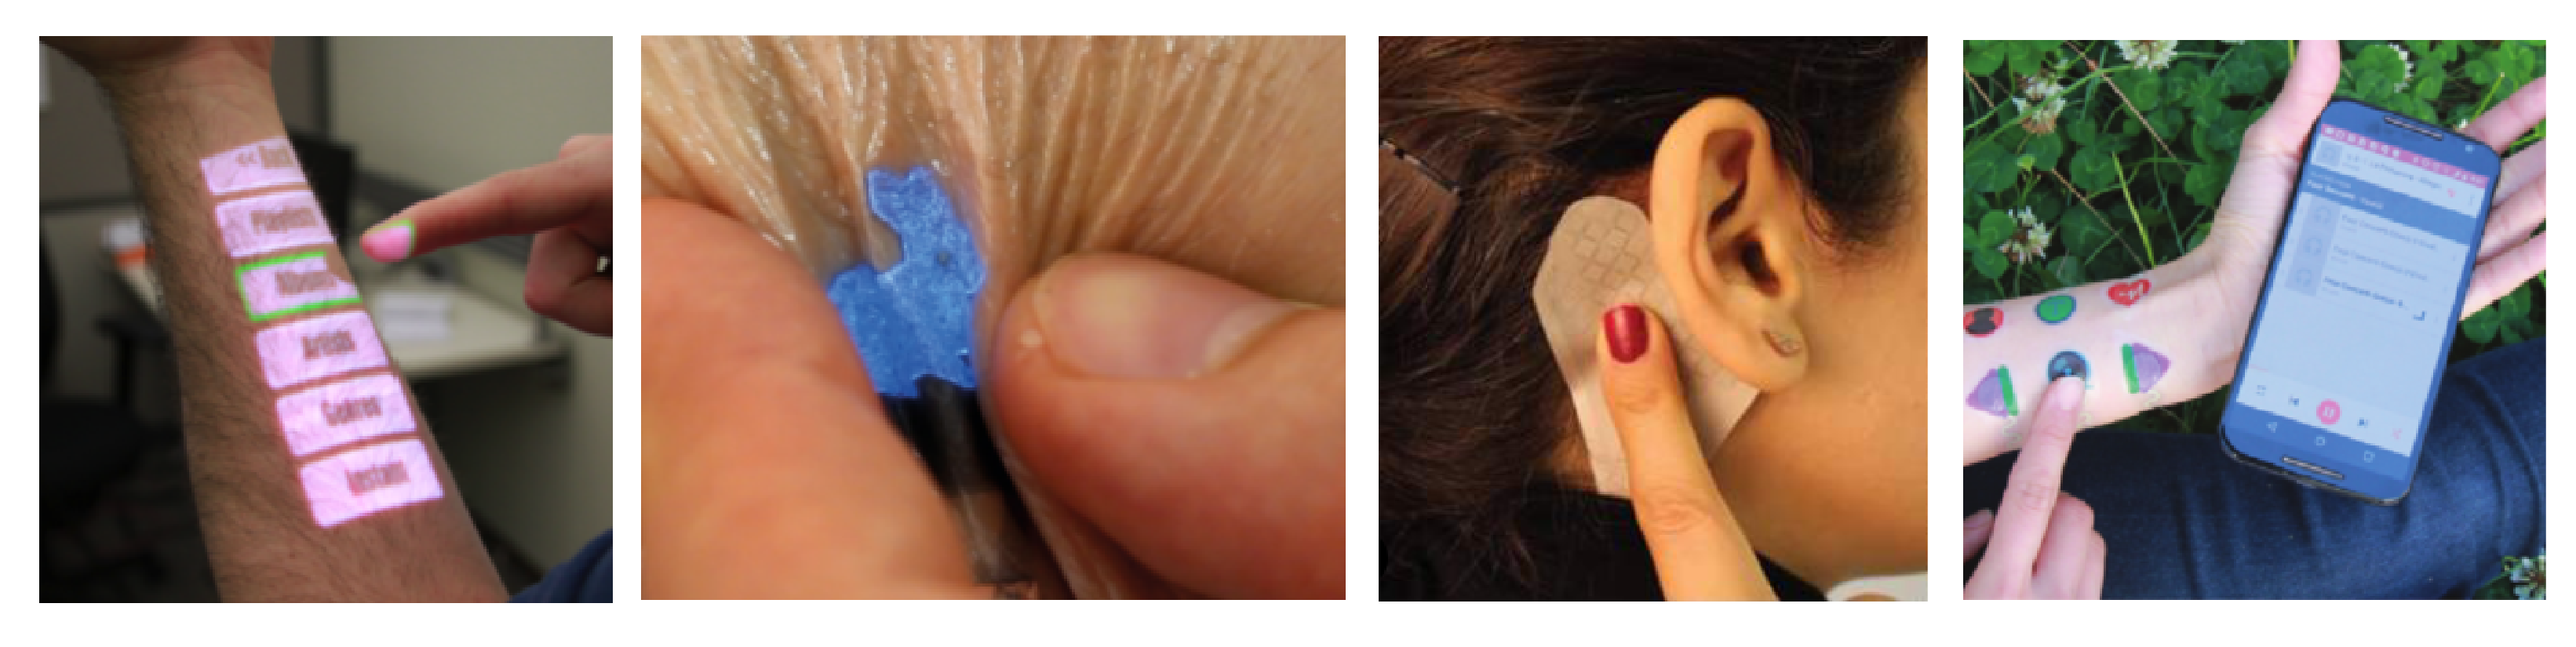
\includegraphics[scale=0.55]{pictures/onskin-01.png}
    \caption{An example of different on-skin interfaces. From left to right:\\ Omnitouch \cite{Harrison:2011:OWM:2047196.2047255}, SkinMarks \cite{Weigel:2017:SEI:3025453.3025704}, Multi-touch skin \cite{Nittala:2018:MST:3173574.3173607} and Skintillates \cite{Lo:2016:SDC:2901790.2901885}.
    }
    \label{fig:intro_sensors}
\end{figure}

As new forms of 3D printing and digital fabrication emerge, it is important to leverage automatized tools that are capable to ease this process for the user. In more detail, it is necessary to provide the ability to create designs that are easily replicable, shareable with others, archivable, fabricated remotely and adaptable to different bodies \cite{Gannon:2016:EOF:2858036.2858576}.\\
Additionally, there is a potential market to attract the audience - without technical background - to design and customize their own products. Such personalization is especially interesting for producing objects which adapt perfectly on a user's body such as braces, jewelry and other wearable devices.\newpara
Since the idea of producing touch sensors for the human skin is a rather recent discovery in human-computer interaction ( HCI ), very few design tools have been developed up to this day. 
It is hence important to introduce the first step towards the larger vision of easy customization and prototyping of on-body devices.

\subsection{Our approach}
We propose a digital design application (viz., Scansify) which enables users to create a design layout and then fabricate on-skin sensors \cite{Nittala:2018:MST:3173574.3173607} that conform to the user’s body. In our case, we have decided to focus on the arm part of the human body as it provides an easily accessible surface and is generally the most favorable area on the body for touch interfaces \cite{Harrison:2012:OIA:2148131.2148148, Harrison:2014:ILT:2598510.2598587}. Using a handheld depth sensor camera, our digital framework scans the outer form of the human figure and allows the user to digitally draw on the reconstructed model. After the drawing process, the input forwards into a post-processing pipeline and converts to a flat 2D shape which can be used for creating sensors (see \textbf{\autoref{subsec:overview}}).\\
After fabricating, the overlay wraps perfectly on the user's arm the way it was previously designed by the user (see \textbf{\autoref{fig:intro_tool}}).\\

\begin{figure}[H]
    \captionit
    \centering
    
\includegraphics[scale=0.65]{pictures/placeholder.png}
    \caption{An example of the work flow of Scansify.\\
    a) Drawing the layout in 3D;\\
    b) Our tool outputs a 2D shape which can be further processed;\\
    c) The shape fits perfectly on the skin
    }
    \label{fig:intro_tool}
\end{figure}

Scansify provides guidance, feedback, and support of various other operations. The following list summarizes the key implemented contribution of this thesis:\newpara
\label{item:functionality}
\textbf{Primary:} The core functionality
\begin{itemize} 
\item[\textbf{a)}] Capturing the human body with a RGB-D camera for acquiring precise geometry.
\item[\textbf{b)}] Live display of skin reconstruction process and depth stream from the camera.
\item[\textbf{c)}] Ability to annotate the digital body with a graphical user interface.
\item[\textbf{d)}] Unwrap algorithm that transforms the 3D drawing into a 2D shape.\\
\end{itemize}
\textbf{Secondary:} The remaining functionality that improves usability
\begin{itemize} 
\item[\textbf{e)}] Import and export of designs and 3d models.
\item[\textbf{f)}] Revert of latest change or completely reset the design.
\item[\textbf{g)}] Manipulation of camera view (steering, zooming or rotating).\newpara\\
\end{itemize}
Our approach especially target users that are not familiar with designing on-body sensors by providing an intuitive product for rapid prototyping. At the end, a use-case study is conducted and results are discussed to evaluate the feasibility and usability of the product. In addition, feedback is taken to refine the design principles for future iterations.
\subsection{Structure of the thesis}
The following list depicts a short overview of the subjects covered in the remaining chapters:
\paragraph*{\hyperref[sec:relatedwork]{Chapter 2}} presents recent work in on-body interaction and depth-sensing advances.
\paragraph*{\hyperref[sec:goals]{Chapter 3}} introduces the main concept and novel design considerations as a result of the related work chapter.
\paragraph*{\hyperref[sec:implementation]{Chapter 4}} illustrates a detailed workflow description of the graphical user interface and outlines the development process of Scansify.
\paragraph*{\hyperref[sec:results]{Chapter 5}} evaluates the results from a user study with respect to the feasibility and usability of our tool.
\paragraph*{\hyperref[sec:discussion]{Chapter 6}} concludes the thesis with a discussion on limitation and approaches for future work.

\newpage
\thispagestyle{empty}